\documentclass{article}
\usepackage{graphicx} % Required for inserting images
\usepackage{tikz}
\usepackage{amsthm}
\usepackage{amssymb}
\usepackage{mathtools}
\usepackage{hyperref}

\usepackage{pgfplots}
\pgfplotsset{width=10cm,compat=1.9}
\usepackage{mathpazo}
\usepackage{fp}
\newcounter{row}
\newcounter{col}

\newcommand\setrow[9]{
  \setcounter{col}{1}
  \foreach \n in {#1, #2, #3, #4, #5, #6, #7, #8, #9} {
    \edef\x{\value{col} - 0.5}
    \edef\y{9.5 - \value{row}}
    \node[anchor=center] at (\x, \y) {\huge \n};
    \stepcounter{col}
  }
  \stepcounter{row}
}

\newcommand{\drawrectcage}[5]{
    %coordinates of SW, then NE of rectangle
    \draw[dashed] (#1 + 0.1, #2 + 0.1) rectangle (#3 - 0.1, #4 - 0.1);

    \node[rectangle, draw=white, fill=white, minimum size=6pt] at (#1 + 1.5, #4 - 0.5) {#5};
}

\title{Parallel Sudoku Solver}
\author{Liam Gersten (lgersten) and Alexander Wang (aywang)}

\begin{document}

\maketitle

\centering
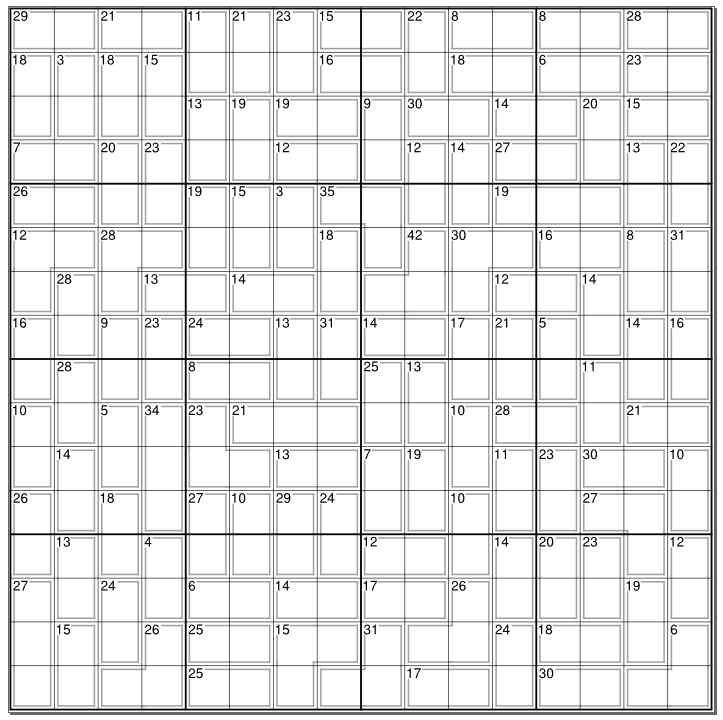
\includegraphics[width=1.0\linewidth]{images/sudoku_example.png}
\newpage

\section{A Sat Reduction}
\begin{figure}[!htb]
    \centering
    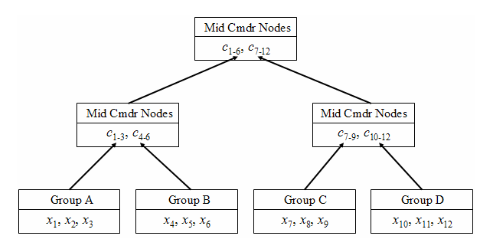
\includegraphics[width=1\linewidth]{images/comm1.png}
    \caption{Graphical Depiction of Commander Variable Encoding}
\end{figure}

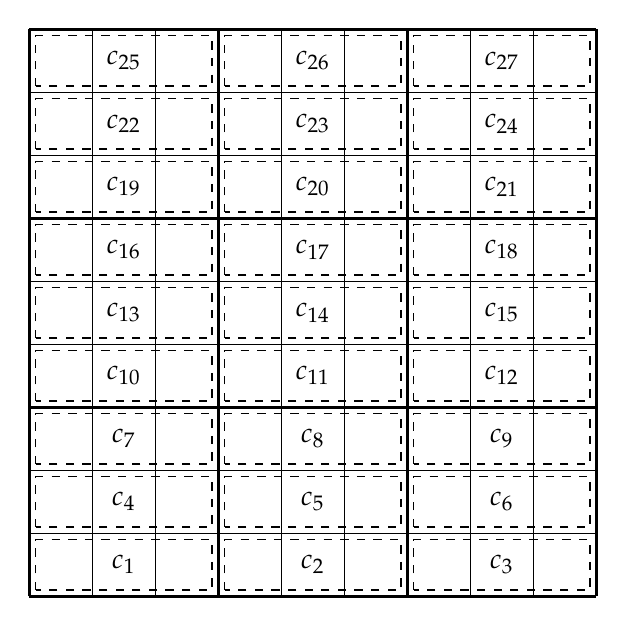
\begin{tikzpicture}[scale=.8]

  \begin{scope}
    \draw (0, 0) grid (9, 9);
    \draw[very thick, scale=3] (0, 0) grid (3, 3);

    \setcounter{row}{1}
    \setrow { }{ }{ }  { }{ }{ }  { }{ }{ }
    \setrow { }{ }{ }  { }{ }{ }  { }{ }{ }
    \setrow { }{ }{ }  { }{ }{ }  { }{ }{ }

    \setrow { }{ }{ }  { }{ }{ }  { }{ }{ }
    \setrow { }{ }{ }  { }{ }{ }  { }{ }{ }
    \setrow { }{ }{ }  { }{ }{ }  { }{ }{ }

    \setrow { }{ }{ }  { }{ }{ }  { }{ }{ }
    \setrow { }{ }{ }  { }{ }{ }  { }{ }{ }
    \setrow { }{ }{ }  { }{ }{ }  { }{ }{ }
  \end{scope}
  
  \drawrectcage{0}{0}{3}{1}{$c_1$};
  \drawrectcage{3}{0}{6}{1}{$c_2$};
  \drawrectcage{6}{0}{9}{1}{$c_3$};
  \drawrectcage{0}{1}{3}{2}{$c_4$};
  \drawrectcage{3}{1}{6}{2}{$c_5$};
  \drawrectcage{6}{1}{9}{2}{$c_6$};
  \drawrectcage{0}{2}{3}{3}{$c_7$};
  \drawrectcage{3}{2}{6}{3}{$c_8$};
  \drawrectcage{6}{2}{9}{3}{$c_9$};
  \drawrectcage{0}{3}{3}{4}{$c_{10}$};
  \drawrectcage{3}{3}{6}{4}{$c_{11}$};
  \drawrectcage{6}{3}{9}{4}{$c_{12}$};
  \drawrectcage{0}{4}{3}{5}{$c_{13}$};
  \drawrectcage{3}{4}{6}{5}{$c_{14}$};
  \drawrectcage{6}{4}{9}{5}{$c_{15}$};
  \drawrectcage{0}{5}{3}{6}{$c_{16}$};
  \drawrectcage{3}{5}{6}{6}{$c_{17}$};
  \drawrectcage{6}{5}{9}{6}{$c_{18}$};
  \drawrectcage{0}{6}{3}{7}{$c_{19}$};
  \drawrectcage{3}{6}{6}{7}{$c_{20}$};
  \drawrectcage{6}{6}{9}{7}{$c_{21}$};
  \drawrectcage{0}{7}{3}{8}{$c_{22}$};
  \drawrectcage{3}{7}{6}{8}{$c_{23}$};
  \drawrectcage{6}{7}{9}{8}{$c_{24}$};
  \drawrectcage{0}{8}{3}{9}{$c_{25}$};
  \drawrectcage{3}{8}{6}{9}{$c_{26}$};
  \drawrectcage{6}{8}{9}{9}{$c_{27}$};

\end{tikzpicture}

\begin{align*}
    &[\text{digitInCage}] \iff \bigwedge_{\text{cell} \in \text{cage}} [\text{digitInCell}] \tag{1}\\
    &[\text{validPartition}] \iff \bigwedge_{\text{digit} \in \text{partition}} [\text{digitInCage}] \tag{2}\\
    &\bigvee_{\text{all partitions with valid sum}} [\text{validPartition}] \tag{3}
\end{align*}

\newpage

\section{Recursive Algorithm}
\vspace*{\fill}
\begin{center}
    \begin{tikzpicture}
        \begin{scope}[every node/.style={circle,thick,draw}]
            \node (R) at (8, 6) {$S_0$};
            \node (S1T) at (3, 2) {$S_1$};
            \node (S1F) [dashed, draw=gray, thin, text=gray] at (13, 2) {$S_1'$} ;
            \node (S2T) [draw=orange, thin, text=orange] at (1, -2) {$S_2$};
            \node (S2F) at (7, -2) {$S_2'$} ;
            \node (S3T) at (4, -6) {$S_3$};
            \node (S3F) [dashed, draw=gray, thin, text=gray] at (10, -6) {$S_3'$} ;
        \end{scope}
        
        \begin{scope}[
                      every node/.style={fill=white,circle},
                      every edge/.style={draw=black,very thick}]
            \path [->] (R) edge[bend right=30] node {$x_1 = T$} (S1T);
            \path [->] (R) edge[bend left=30, dashed, draw=gray, thin, text=gray] node {$x_1 = F$} (S1F);
            \path [->] (S1T) edge[bend right=30, draw=orange, thin, text=orange] node {$x_2 = T$} (S2T);
            \path [->] (S1T) edge[bend left=30] node {$x_2 = F$} (S2F);
            \path [->] (S2F) edge[bend right=30] node {$x_3 = T$} (S3T);
            \path [->] (S2F) edge[bend left=30, dashed, draw=gray, thin, text=gray] node {$x_3 = F$} (S3F);
        \end{scope}
    \end{tikzpicture}
\end{center}
\vspace*{\fill}
\newpage

\section{How to Steal Things}

\vspace*{\fill}
\begin{center}
    \begin{tikzpicture}
        \begin{scope}[every node/.style={rectangle,thick,draw}]
            \node (l0) [draw=black, text=black] at (8, 4.5) {PID 0} ;
        \end{scope}
        \begin{scope}[every node/.style={circle,thick,draw}]
            \node (R) [draw=red, text=red] at (8, 3) {$S_0$};
            \node (S1T) [draw=red, text=red] at (4, 1) {$S_1$};
            \node (S1F) [dashed, thin, draw=blue, text=blue] at (12, 1) {$S_1'$} ;
            \node (S2T) [draw=red, thin, text=red] at (2, -1) {$S_2$};
            \node (S2F) at (7, -1) {$S_2'$} ;
            \node (S3T) at (5, -3) {$S_3$};
            \node (S3F) [dashed, draw=gray, thin, text=gray] at (9, -3) {$S_3'$} ;
        \end{scope}
        
        \begin{scope}[
                      every node/.style={fill=white,circle},
                      every edge/.style={draw=black,very thick}]
            \path [->] (R) edge[bend right=20, draw=red, text=red] node {$x_1 = T$} (S1T);
            \path [->] (R) edge[bend left=20, dashed, draw=blue, thin, text=blue] node {$x_1 = F$} (S1F);
            \path [->] (S1T) edge[bend right=20, draw=red, thin, text=red] node {$x_2 = T$} (S2T);
            \path [->] (S1T) edge[bend left=20, draw=red, text=red] node {$x_2 = F$} (S2F);
            \path [->] (S2F) edge[bend right=20] node {$x_3 = T$} (S3T);
            \path [->] (S2F) edge[bend left=20, dashed, draw=gray, thin, text=gray] node {$x_3 = F$} (S3F);
        \end{scope}
    \end{tikzpicture}
\end{center}
\vspace*{\fill}
\begin{center}
    \begin{tikzpicture}
        \begin{scope}[every node/.style={rectangle,thick,draw}]
            \node (l0) [draw=black, text=black] at (4, 2.5) {PID 0} ;
            \node (l1) [draw=blue, text=blue] at (12, 2.5) {PID 1} ;
        \end{scope}
        \begin{scope}[every node/.style={circle,thick,draw}]
            \node (S1F) [draw=blue, text=blue] at (12, 1) {$S_1'$} ;
            \node (S2F) at (4, 1) {$S_2'$} ;
            \node (S3T) at (2, -1) {$S_3$};
            \node (S3F) [dashed, draw=gray, thin, text=gray] at (6, -1) {$S_3'$} ;
        \end{scope}
        
        \begin{scope}[
                      every node/.style={fill=white,circle},
                      every edge/.style={draw=black,very thick}]
            \path [->] (S2F) edge[bend right=20] node {$x_3 = T$} (S3T);
            \path [->] (S2F) edge[bend left=20, dashed, draw=gray, thin, text=gray] node {$x_3 = F$} (S3F);
        \end{scope}
    \end{tikzpicture}
\end{center}
\vspace*{\fill}
\newpage

\section{Public Speaking}
\vspace*{\fill}
\begin{center}
    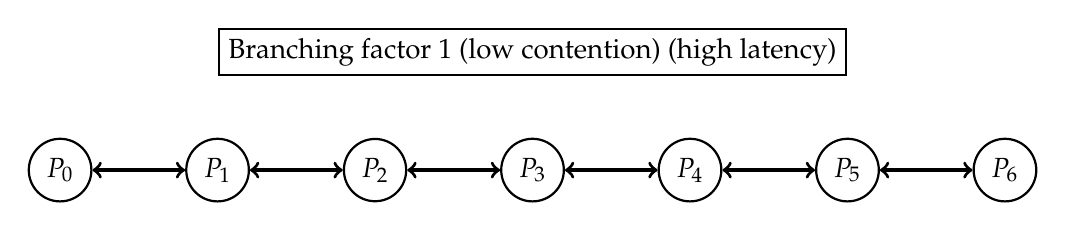
\begin{tikzpicture}
        \begin{scope}[every node/.style={rectangle,thick,draw}]
            \node (l0) [draw=black, text=black] at (8, 1.5) {Branching factor 1 (low contention) (high latency)} ;
        \end{scope}
        \begin{scope}[every node/.style={circle,thick,draw}]
            \node (P0) at (2, 0) {$P_0$};
            \node (P1) at (4, 0) {$P_1$};
            \node (P2) at (6, 0) {$P_2$};
            \node (P3) at (8, 0) {$P_3$};
            \node (P4) at (10, 0) {$P_4$};
            \node (P5) at (12, 0) {$P_5$};
            \node (P6) at (14, 0) {$P_6$};
        \end{scope}
        \path [<->] (P0) edge[draw=black,very thick] node {} (P1);
        \path [<->] (P1) edge[draw=black,very thick] node {} (P2);
        \path [<->] (P2) edge[draw=black,very thick] node {} (P3);
        \path [<->] (P3) edge[draw=black,very thick] node {} (P4);
        \path [<->] (P4) edge[draw=black,very thick] node {} (P5);
        \path [<->] (P5) edge[draw=black,very thick] node {} (P6);
    \end{tikzpicture}
\end{center}
\vspace*{\fill}
\begin{center}
    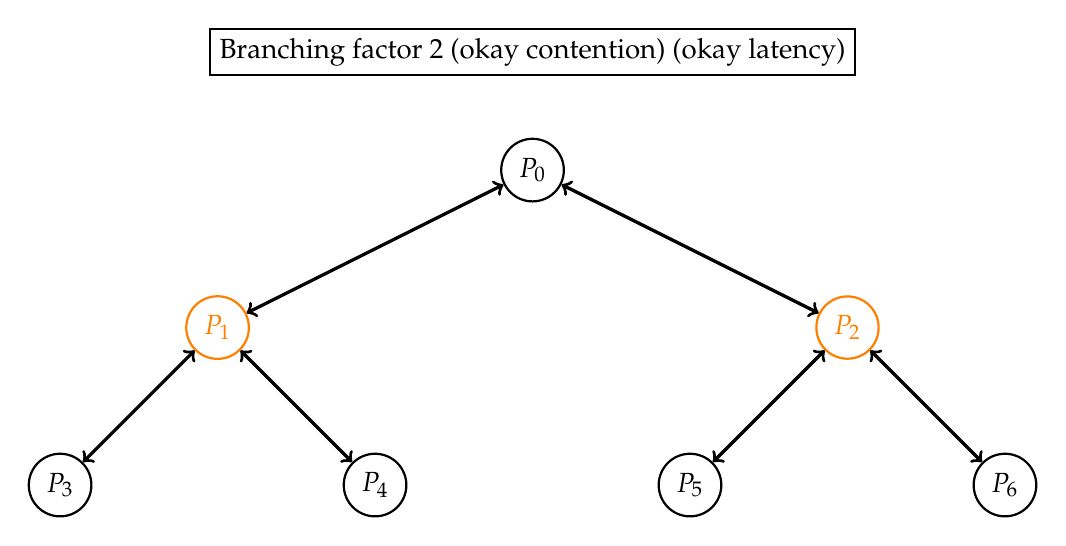
\begin{tikzpicture}
        \begin{scope}[every node/.style={rectangle,thick,draw}]
            \node (l0) [draw=black, text=black] at (8, 5.5) {Branching factor 2 (okay contention) (okay latency)} ;
        \end{scope}
        \begin{scope}[every node/.style={circle,thick,draw}]
            \node (P0) at (8, 4) {$P_0$};
            \node (P1) [draw=orange, text=orange] at (4, 2) {$P_1$};
            \node (P2) [draw=orange, text=orange] at (12, 2) {$P_2$};
            \node (P3) at (2, 0) {$P_3$};
            \node (P4) at (6, 0) {$P_4$};
            \node (P5) at (10, 0) {$P_5$};
            \node (P6) at (14, 0) {$P_6$};
        \end{scope}
        \path [<->] (P0) edge[draw=black,very thick] node {} (P1);
        \path [<->] (P0) edge[draw=black,very thick] node {} (P2);
        \path [<->] (P1) edge[draw=black,very thick] node {} (P3);
        \path [<->] (P1) edge[draw=black,very thick] node {} (P4);
        \path [<->] (P2) edge[draw=black,very thick] node {} (P5);
        \path [<->] (P2) edge[draw=black,very thick] node {} (P6);
    \end{tikzpicture}
\end{center}
\vspace*{\fill}
\begin{center}
    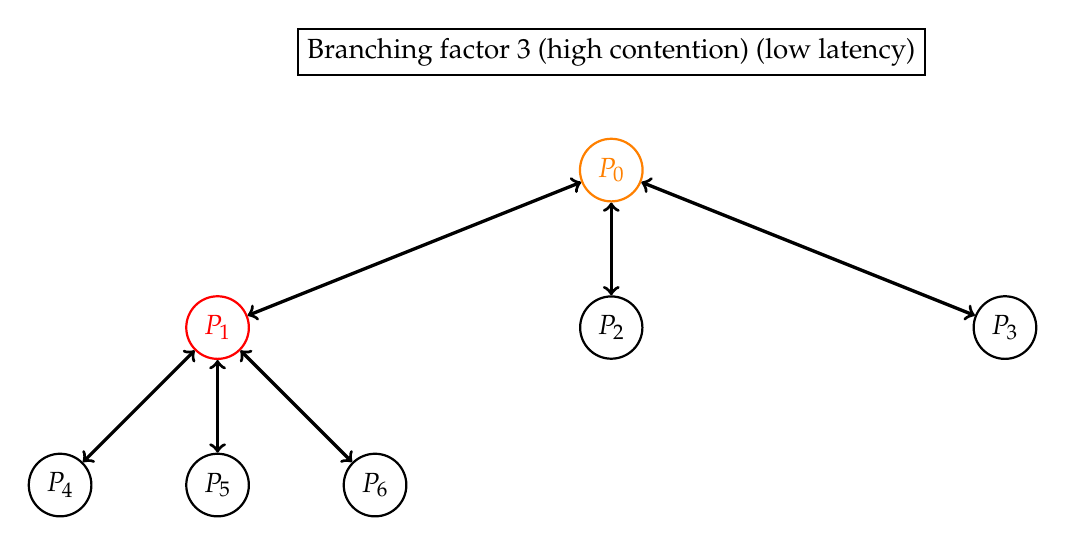
\begin{tikzpicture}
        \begin{scope}[every node/.style={rectangle,thick,draw}]
            \node (l0) [draw=black, text=black] at (8, 5.5) {Branching factor 3 (high contention) (low latency)} ;
        \end{scope}
        \begin{scope}[every node/.style={circle,thick,draw}]
            \node (P0) [draw=orange, text=orange] at (8, 4) {$P_0$};
            \node (P1) [draw=red, text=red] at (3, 2) {$P_1$};
            \node (P2) at (8, 2) {$P_2$};
            \node (P3) at (13, 2) {$P_3$};
            \node (P4) at (1, 0) {$P_4$};
            \node (P5) at (3, 0) {$P_5$};
            \node (P6) at (5, 0) {$P_6$};
        \end{scope}
        \path [<->] (P0) edge[draw=black,very thick] node {} (P1);
        \path [<->] (P0) edge[draw=black,very thick] node {} (P2);
        \path [<->] (P0) edge[draw=black,very thick] node {} (P3);
        \path [<->] (P1) edge[draw=black,very thick] node {} (P4);
        \path [<->] (P1) edge[draw=black,very thick] node {} (P5);
        \path [<->] (P1) edge[draw=black,very thick] node {} (P6);
    \end{tikzpicture}
\end{center}
\vspace*{\fill}
\newpage

\section{Conflict Resolution}
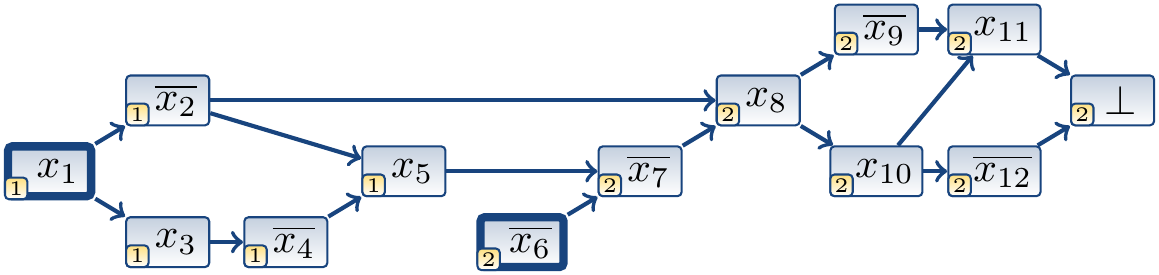
\includegraphics[width=\linewidth]{images/CDCL_1.png}

\vspace{24pt}
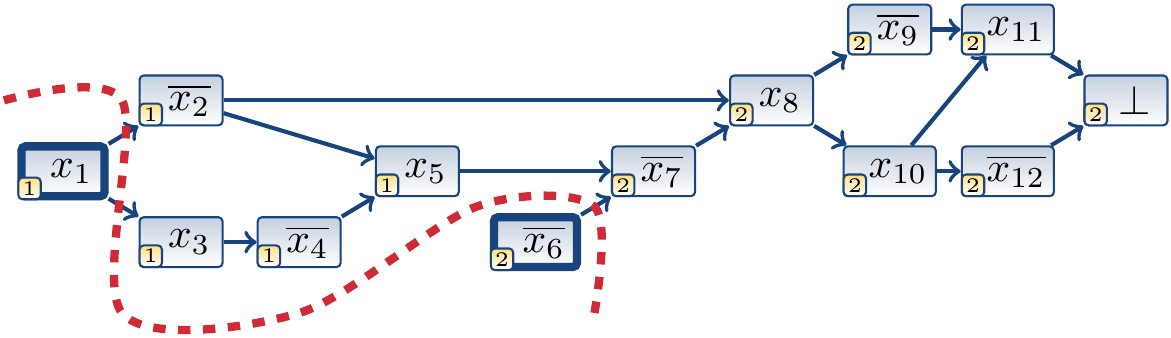
\includegraphics[width=1\linewidth]{images/cc1.png}
\vspace{24pt}
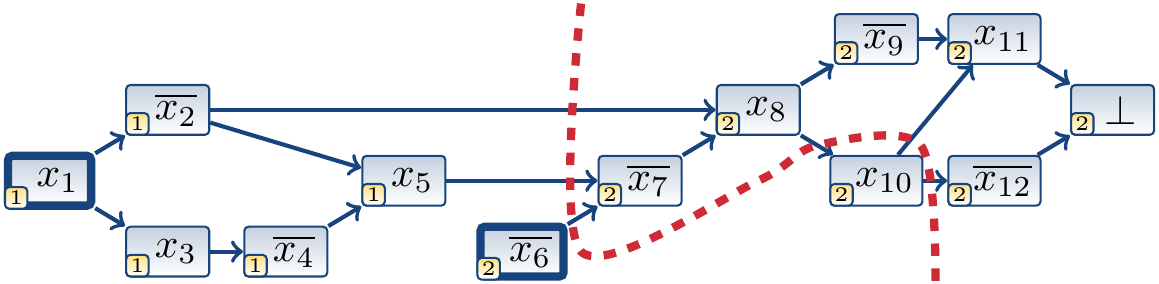
\includegraphics[width=1\linewidth]{images/cc2.png}
\vspace{24pt}
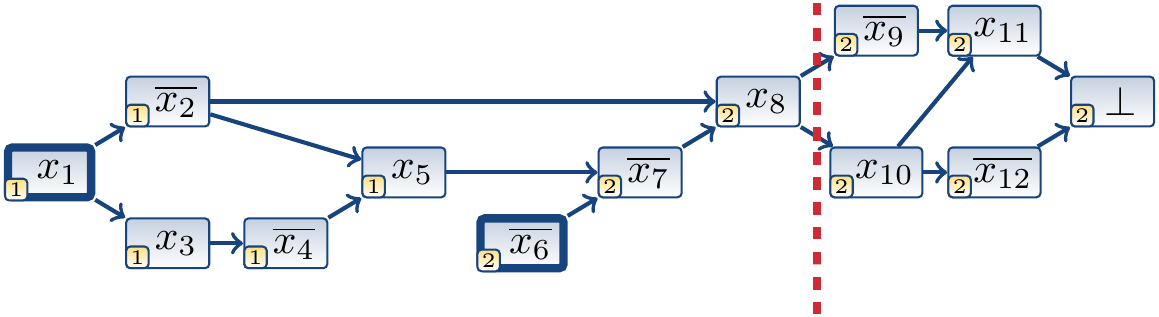
\includegraphics[width=1\linewidth]{images/cc3.png}

\newpage

\section{Performance!}
\vspace*{\fill}
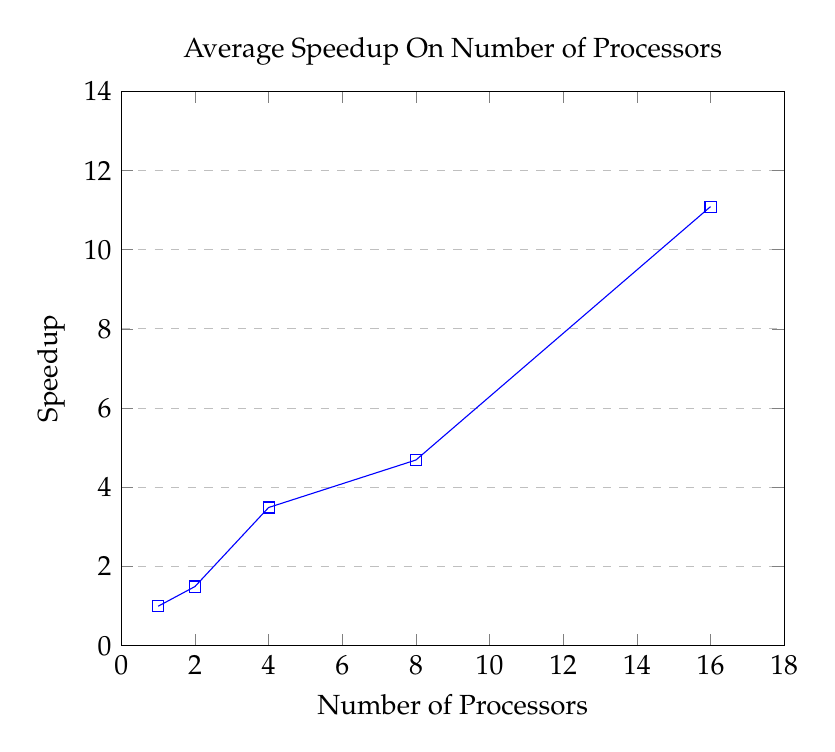
\begin{tikzpicture}
\begin{axis}[
    title={Average Speedup On Number of Processors},
    xlabel={Number of Processors},
    ylabel={Speedup},
    xmin=0, xmax=18,
    ymin=0, ymax=14,
    ymajorgrids=true,
    grid style=dashed,
]
\addplot[
    color=blue,
    mark=square,
    ]
    coordinates {
    (1,1) (2,1.497) (4, 3.492) (8, 4.691) (16,11.088)
    };
    
\end{axis}
\end{tikzpicture}

\vspace{12pt}
\begin{tabular}{c|ccccc}
    \hline
    Puzzle Number & $n=1$ & $n=2$ & $n=4$ & $n=8$ & $n=16$ \\
    \hline
    0 & 29.0 & 89.8 & 16.9 & 1.90 & 1.00\\
    1 & 12.69 & 7.81 & 1.35 & 1.70 & 0.89\\
    2 & 23.66 & 14.5 & 6.88 & 3.85 & 2.96\\
    3 & 4.01 & 2.45 & 1.90 & 2.41 & 0.77
\end{tabular}
\vspace*{\fill}
\newpage

\section{How Perf-ect?}

\begin{figure}[!htb]
    \centering
    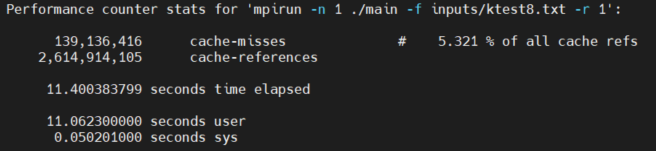
\includegraphics[width=1\linewidth]{images/perf_n1_stat.png}
    \caption{Perf stat on $n=1$ for cache-references and cache-misses.}
\end{figure}
\begin{figure}[!htb]
    \centering
    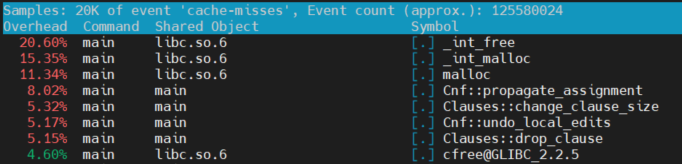
\includegraphics[width=1\linewidth]{images/perf_n1.png}
    \caption{Perf report on $n=1$ for cache-misses}
    \label{fig:perf3}
\end{figure}

\begin{figure}[!htb]
    \centering
    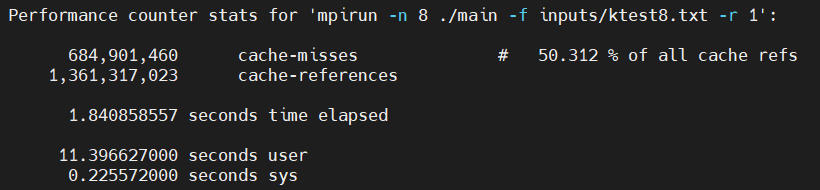
\includegraphics[width=1\linewidth]{images/perf1.png}
    \caption{Perf stat on $n=8$ for cache-references and cache-misses.}
    \label{fig:perf1}
\end{figure}

\begin{figure}[!htb]
    \centering
    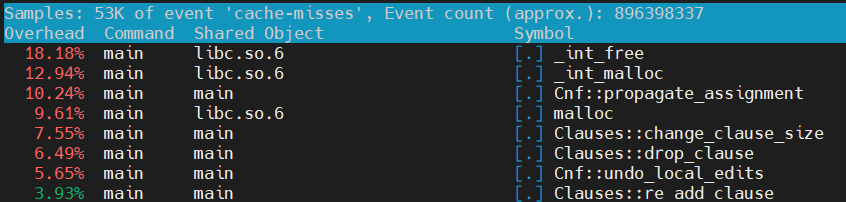
\includegraphics[width=\linewidth]{images/perf2.png}
    \caption{Perf report on $n=8$ for cache-misses}
    \label{fig:perf2}
\end{figure}

\newpage

\end{document}
